\section{Введение}

В 2022-2023 учебном году, комплекты заданий и решений теоретических туров районного, областного и заключительного этапов республиканской олимпиады школьников по химии сопровождались призывом оставить обратную связь о прошедшей олимпиаде, заполнив онлайн опрос, созданный Коллегией. Ссылка на опрос также дублировалась на официальных каналах Коллегии и на (\href{https://ask.bc-pf.org}{форуме Спроси}). В распространении опроса РНПЦ Дарын и Министерство Просвещения РК не принимали никакого участия. В рамках опроса, помимо «существенных» вопросов, ответы на которые проанализированы в других разделах, участники предоставляли демографические данные. Некоторые сводки настолько нас удивили, что мы решили посвятить им отдельную секцию.

Опрос по районному этапу РО прошли 40 участников. Из них 10 (25\%), 15 (37.5\%) и 15 (37.5\%) человек участвовали за 9, 10 и 11 класс соответственно. Распределение по школам следующее:

\begin{table}[ht]
    \centering
    \begin{tabular}{|l|c|c|}
    \hline
    \textbf{Тип школы} & \textbf{Количество} & \textbf{Процент} \\ \hline
    Обычная школа (в городе) & 16 & 40.0\% \\ \hline
    Обычная школа (в селе) & 12 & 30.0\% \\ \hline
    БИЛ & 8 & 20.0\% \\ \hline
    Другая специализированная школа & 2 & 5.0\% \\ \hline
    Частная школа & 2 & 5.0\% \\ \hline
    НИШ & 0 & 0.0\% \\ \hline
    РФМШ & 0 & 0.0\% \\ \hline
    \end{tabular}
    \caption{Типы школ и их распределение на районном этапе РО}
    \label{tab:region-schols}
\end{table}

Стоит заметить, что ученики НИШ и БИЛ не пишут районный этап и проходят сразу на областной, поэтому ответов от учеников НИШ нет. 8 ответов от учеников БИЛ скорее всего предоставлены учениками, которые самостоятельно прорешивали задания районного этапа.

Опрос по областному этапу РО прошли 60 участников. Из них 28 (46.7\%), 17 (28.3\%), и 15 (25.0\%) человек участвовали за 9, 10 и 11 класс соответственно. Распределение по школам следующее:

\begin{table}[ht]
    \centering
    \begin{tabular}{|l|c|c|}
        \hline
        \textbf{Тип школы} & \textbf{Количество} & \textbf{Процент} \\ \hline
        БИЛ & 31 & 51.7\% \\ \hline
        Другая специализированная школа & 11 & 18.3\% \\ \hline
        НИШ & 8 & 13.3\% \\ \hline
        Обычная школа (в городе) & 6 & 10.0\% \\ \hline
        Частная школа & 3 & 5.0\% \\ \hline
        РФМШ & 1 & 1.7\% \\ \hline
        Обычная школа (в селе) & 0 & 0.0\% \\ \hline
    \end{tabular}
    \caption{Типы школ и их распределение на областном этапе РО}
    \label{tab:obl-schools}
\end{table}

Нельзя не заметить практически полное отсутствие ответов от учников из неспециализированных школ. Конечно, 40 и 60 респондентов для этапа, на котором участвуют десятки тысяч (район) и тысячи (область) школьников, могут быть не репрезентативной выборкой. Однако, сложно представить, что ученики из неспециализированных школ, которые участвовали на районном этапе и заполняли опрос, не заполнили бы опрос на областном этапе, если бы они на нем участвовали. Таким образом, Таблица \ref{tab:obl-schools} может указывать на то, что ученики неспециализированных школ в своем большинстве не проходят дальше районного этапа.

Опрос по заключительному этапу РО прошли 32 участника. Из них 9 (28.1\%), 9 (28.1\%) и 14 (43.8\%) человек участвовали за 9, 10 и 11 класс соответственно. Распределение по школам следующее:

\begin{table}[ht]
    \centering
    \begin{tabular}{|l|c|c|}
    \hline
    \textbf{Тип школы} & \textbf{Количество} & \textbf{Процент} \\ \hline
    БИЛ & 15 & 46.9\% \\ \hline
    Другая специализированная школа & 5 & 15.6\% \\ \hline
    Обычная школа (в городе) & 5 & 15.6\% \\ \hline
    НИШ & 4 & 12.5\% \\ \hline
    Частная школа & 2 & 6.3\% \\ \hline
    РФМШ & 1 & 3.1\% \\ \hline
    Обычная школа (в селе) & 0 & 0.0\% \\ \hline
    \end{tabular}
    \caption{Типы школ и их распределение на заключительном этапе РО}
    \label{tab:respa-schools}
\end{table}

\section{Школы, в которых учатся участники РО}
Сгруппируем школы, в которых учатся участники РО, заполнившие опрос по соответствующему этапу (далее эта ремарка будет подразумеваться), в три категории: школа в селе, школа в городе и специализированная школа (включает БИЛ, НИШ, РФМШ).

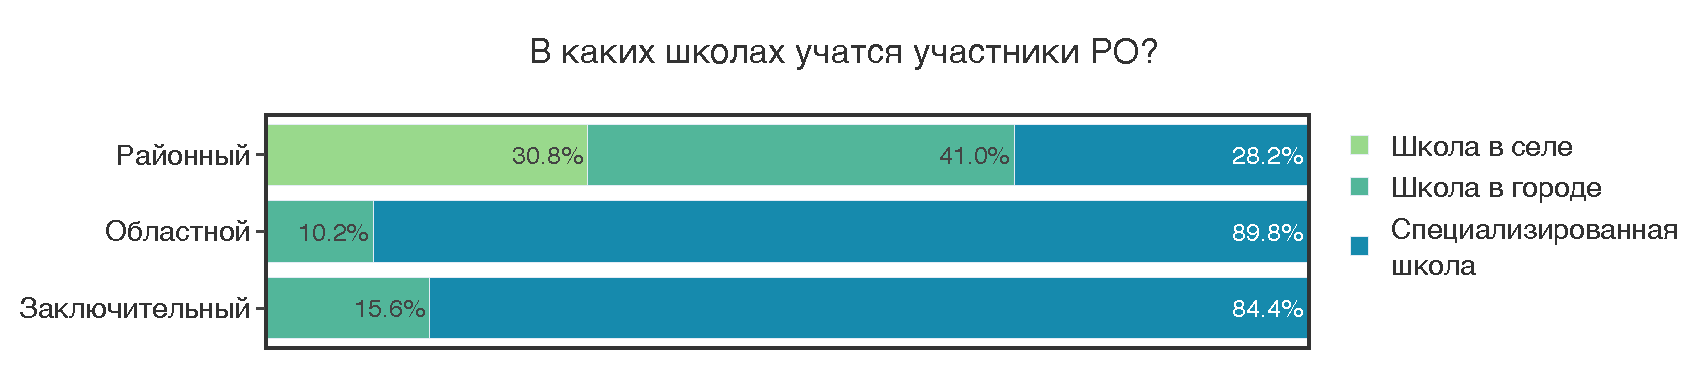
\includegraphics[width=\linewidth]{../export/pdf/demographics/schools.pdf}

\section{Язык обучения и язык участия на РО}

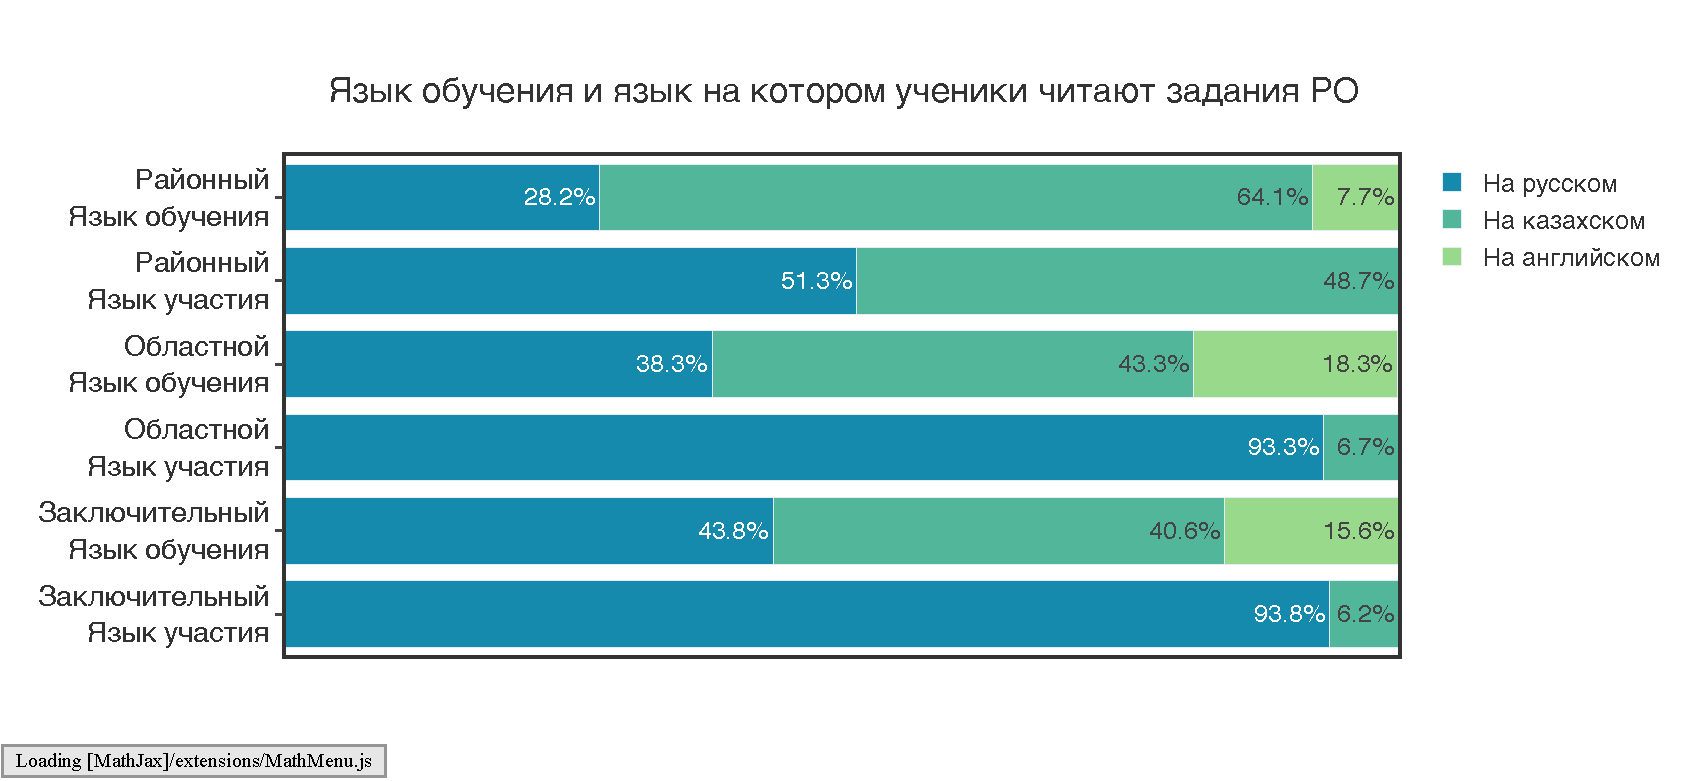
\includegraphics[width=\linewidth]{../export/pdf/demographics/language.pdf}

\section{Пол участников РО}

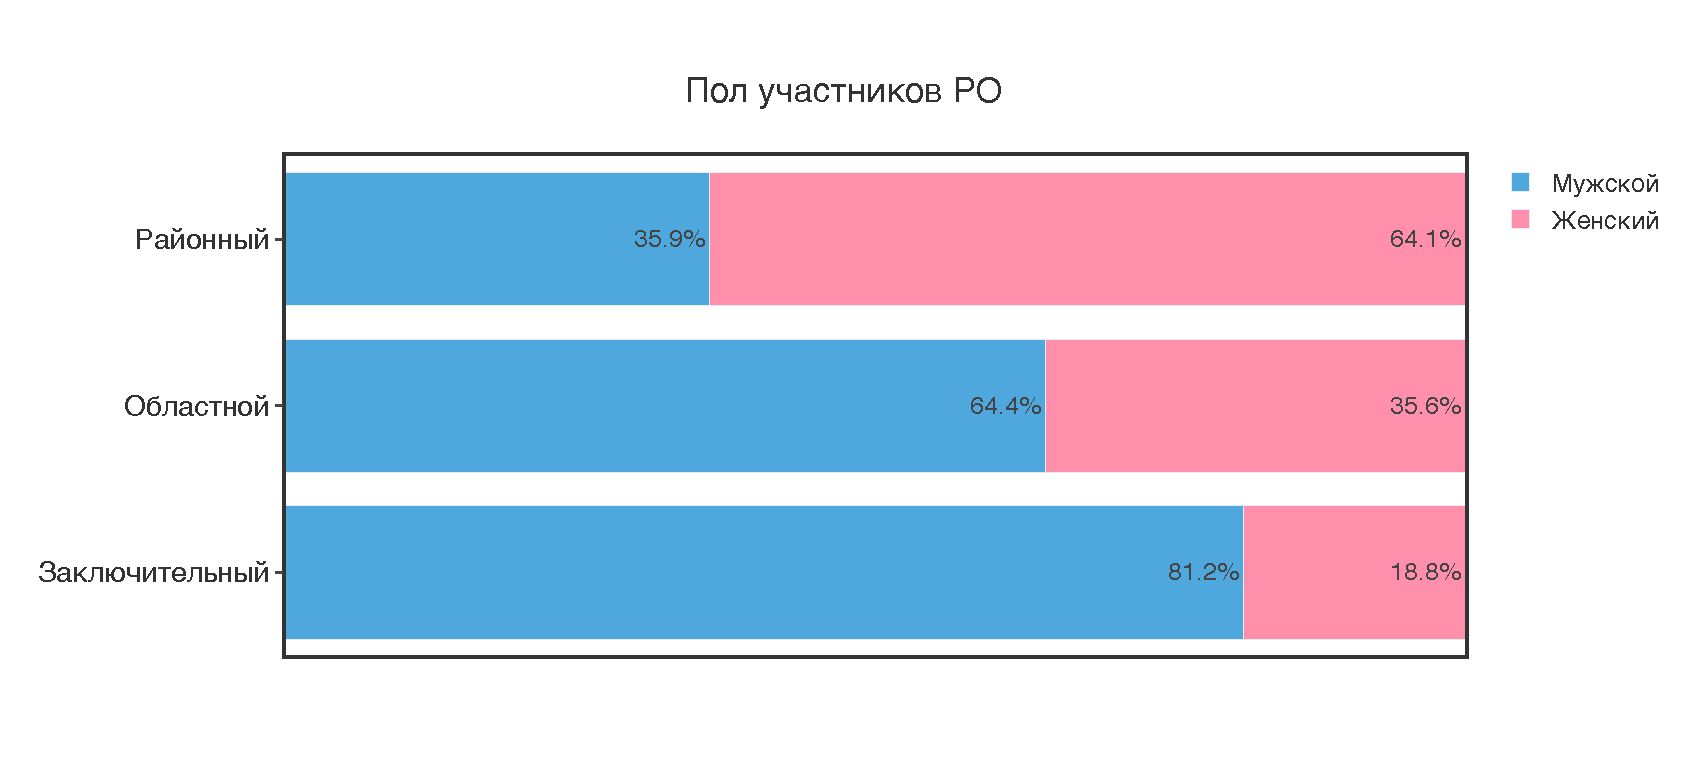
\includegraphics[width=\linewidth]{../export/pdf/demographics/gender.pdf}

\section{Доля участников, участвующих первый раз}

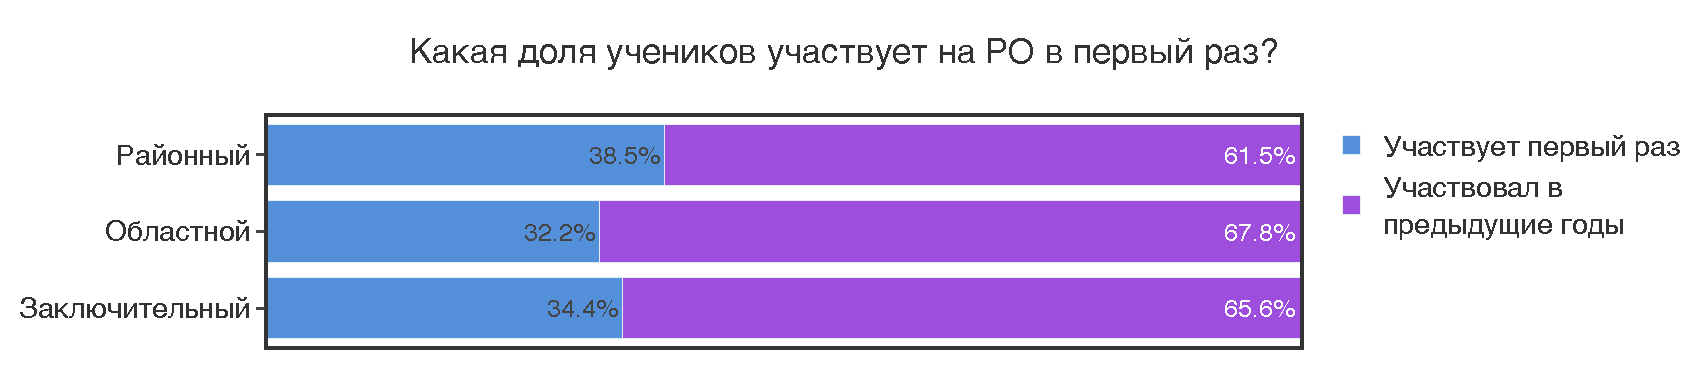
\includegraphics[width=\linewidth]{../export/pdf/demographics/firsttimers.pdf}

Результаты нас удивили. Разумно предположить, что распределение должно зависеть от класса участия: доля участников, участвующих первый раз, должна понижаться в ряду 9, 10, 11 класс. \textit{Примечание:} респонденты должны были ответить на вопрос участвовали ли они первый раз именно на этом этапе РО.

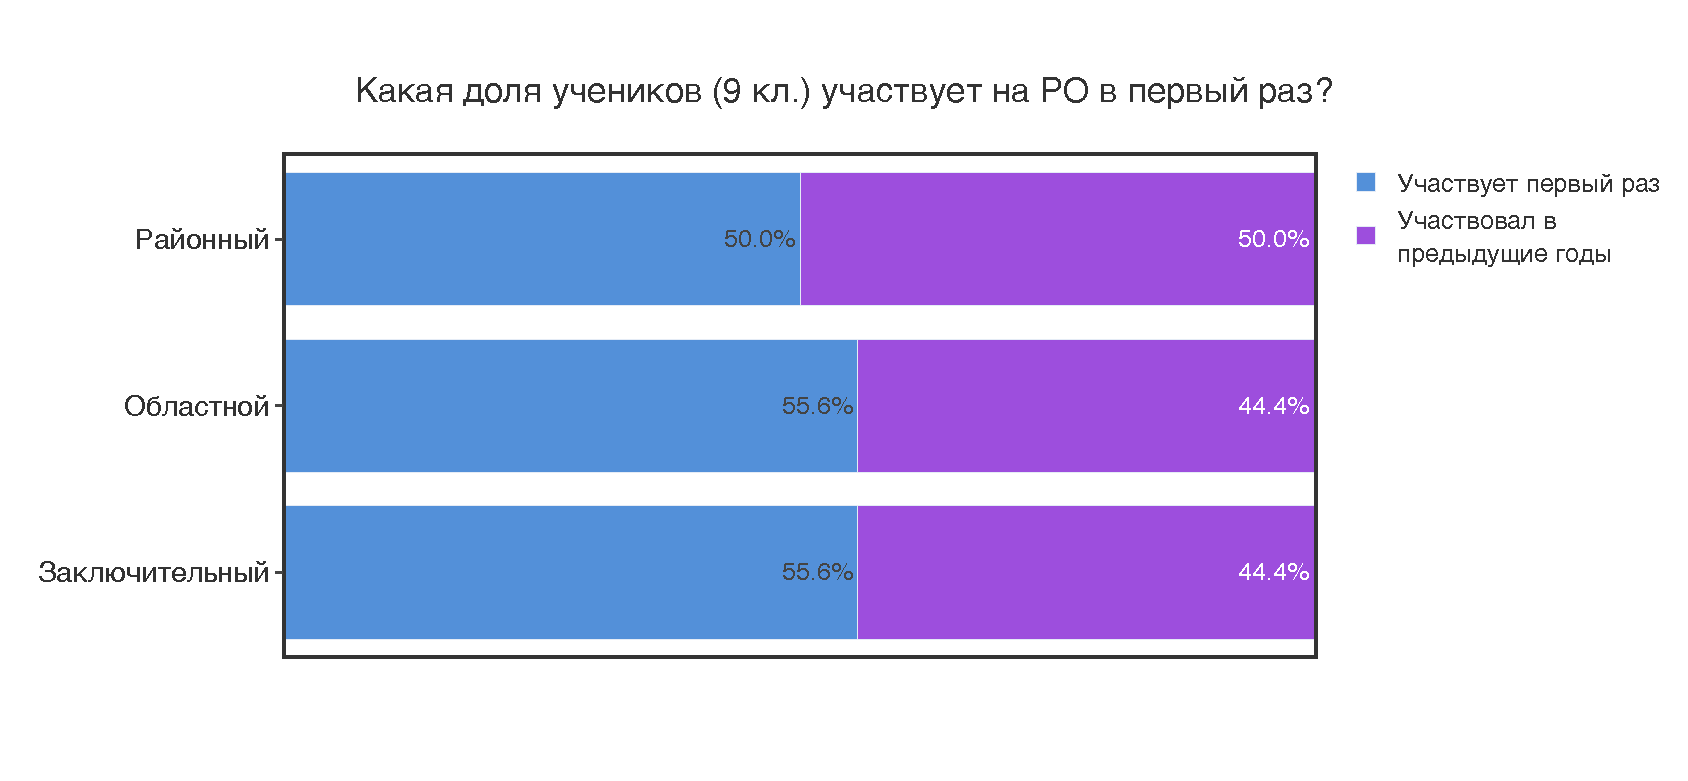
\includegraphics[width=\linewidth]{../export/pdf/demographics/firsttimers-grade9.pdf}

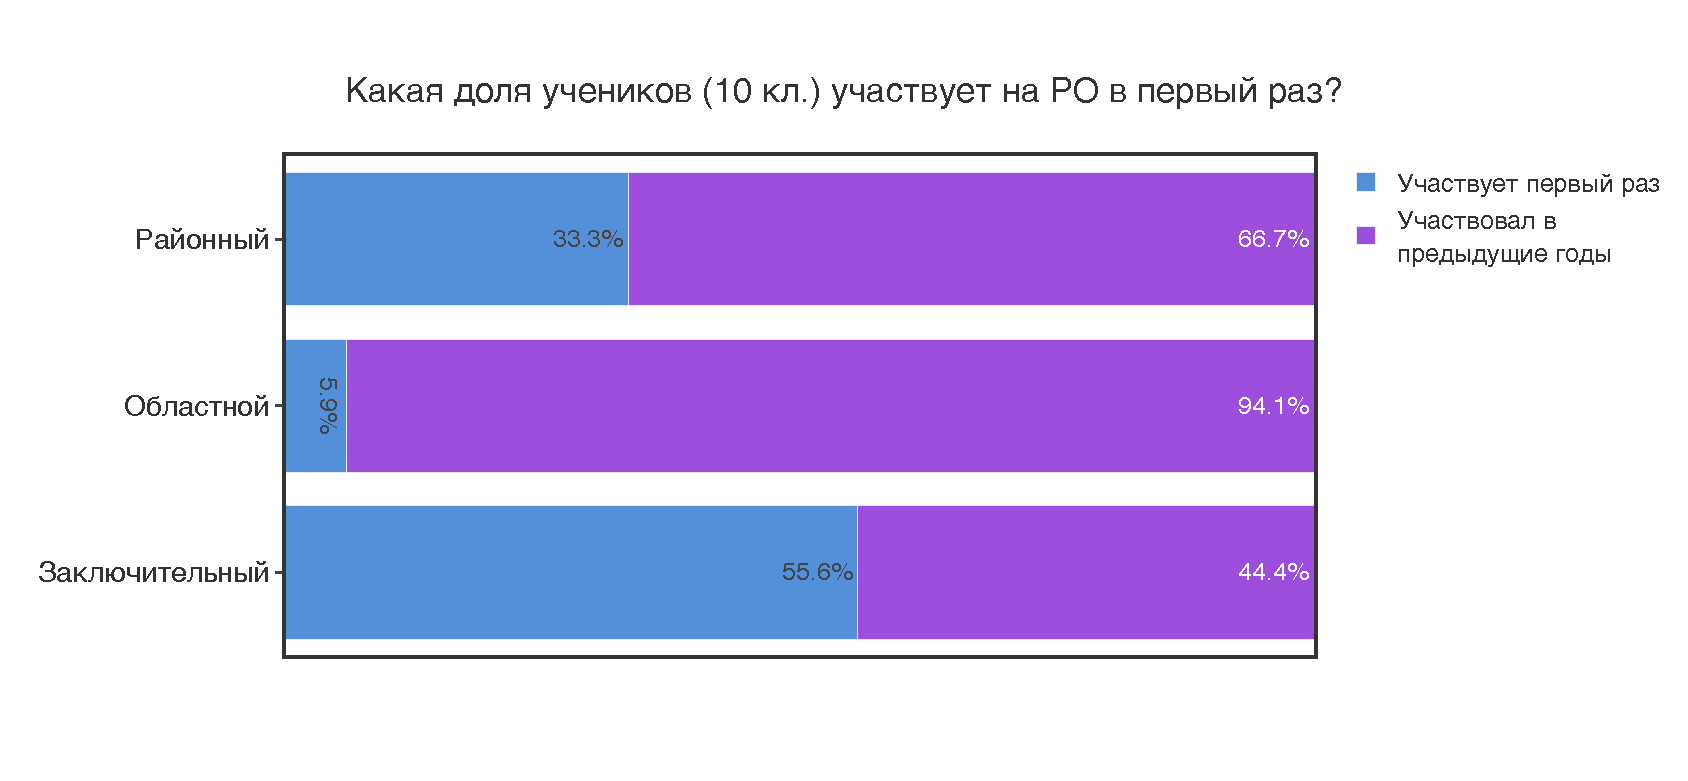
\includegraphics[width=\linewidth]{../export/pdf/demographics/firsttimers-grade10.pdf}

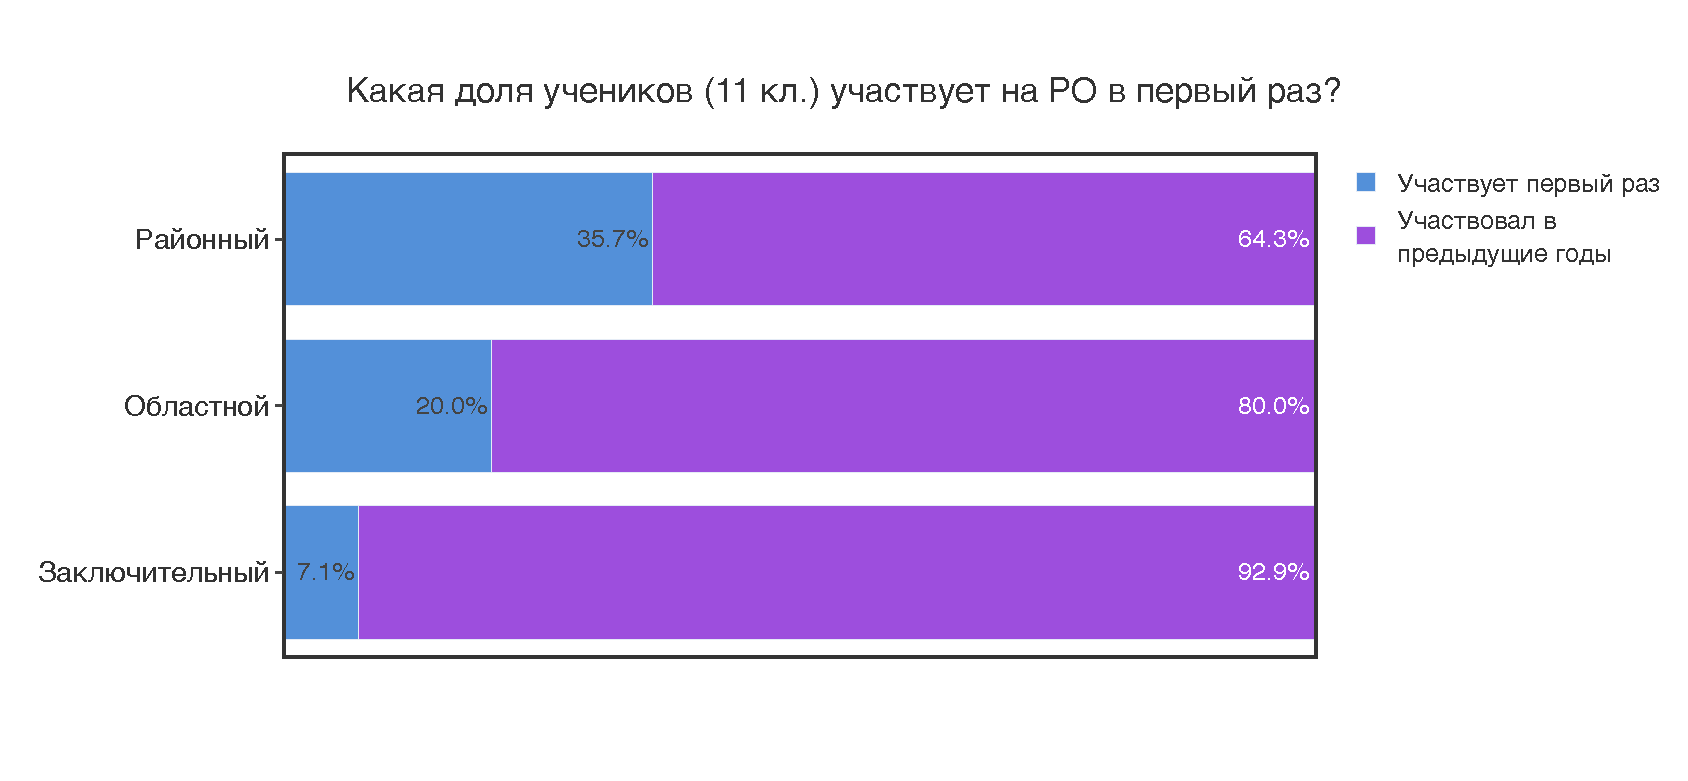
\includegraphics[width=\linewidth]{../export/pdf/demographics/firsttimers-grade11.pdf}

Доля в 50\% тех, кто участвовал в предыдущие годы, среди учеников 9 класса на районном этапе кажется невероятной на первый взгляд. Здесь важно вспомнить, что речь идет о выборке в 10 человек - таким образом, речь идет о 4-5 учениках, что вполне правдоподобное количество. Примечательно, что в 10 классе наблюдается скачок участников, участвующих первый раз, на заключительном этапе по сравнению с областным этапом. Случайно ли это? Связано ли это как-то с заданиями (например, задания были неожиданными для участников, которые участвовали в предыдущие годы, и они были к ним менее готовы.) Не думаем, что размер выборки позволяет дать уверенный ответ, но об этих вопросах, тем не менее, интересно задуматься. 

\section{Длительность подготовки}

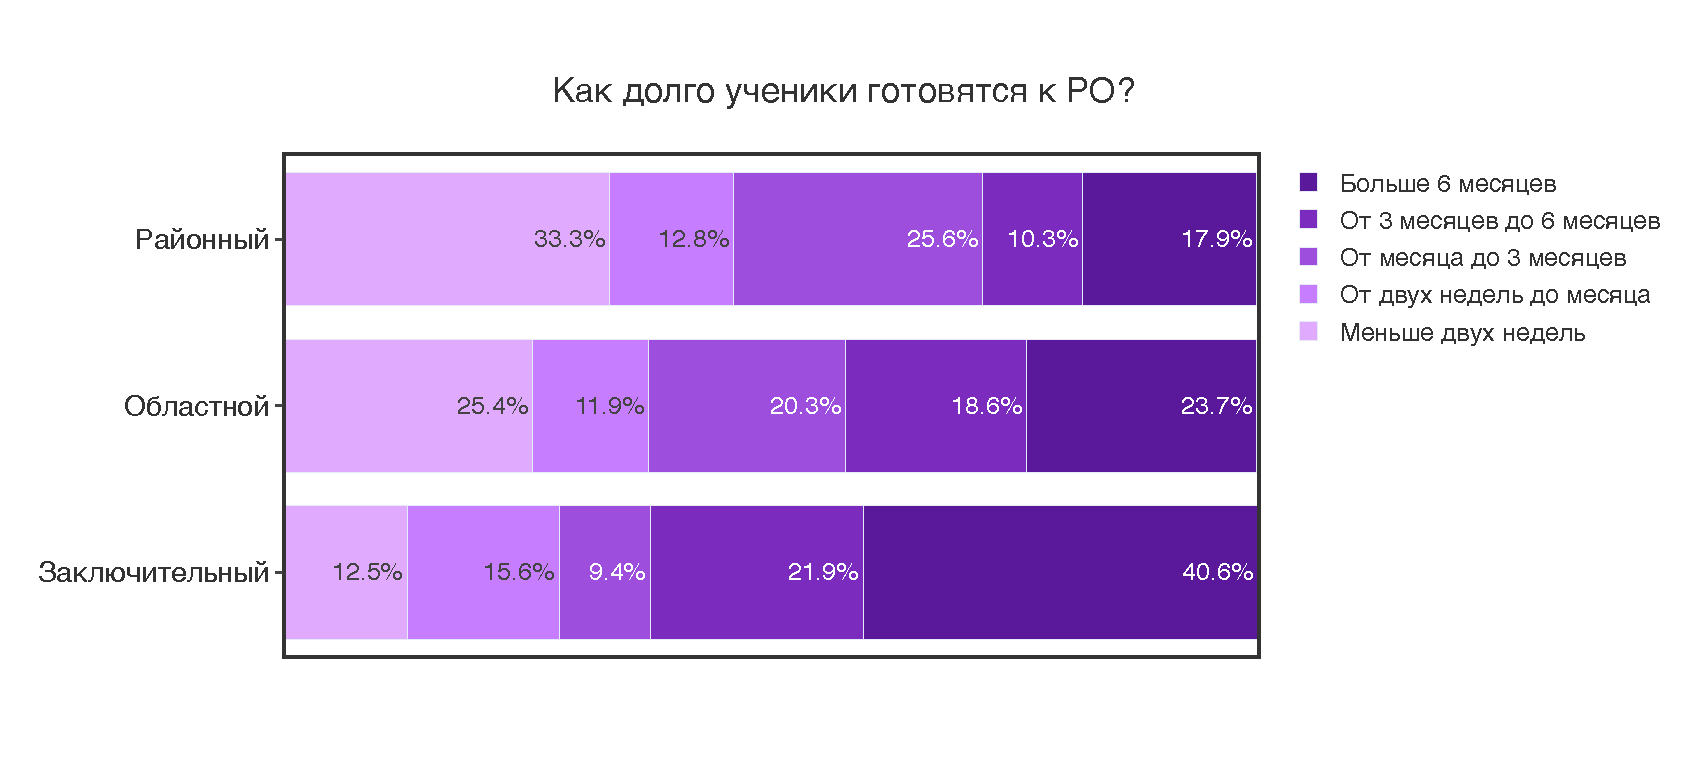
\includegraphics[width=\linewidth]{../export/pdf/demographics/preptime.pdf}

В теории, есть два объяснения этих результатов. Во-первых, областной (заключительный) этап проходит позже районного (областного) и время к его подготовке включает время подготовки к районному (областному) этапу. Во-вторых, на более поздние этапы могут преимущественно проходить те ученики, которые дольше готовятся к олимпиаде. Однако, стоит вспомнить, что районный этап прошел 2 февраля 2023 г., областной этап прошел 13-14 февраля 2023 г., а заключительный этап прошел 21-23 марта 2023 г. Таким образом, разница по времени между этапами была минимальной и разницу в ответах можно объяснить преимущественно второй причиной: на более поздние этапы РО проходят преимущественно те, кто готовится дольше.

\section{Самостоятельно или с учителем?}
Примечательно, что в общественном сознании распространено убеждение, что достижения олимпиадников по большей степени являются заслугой тренеров, которые их готовят. Если определенная область или школа хочет улучшить свои результаты на олимпиадах, первое, что она пытается сделать - найти тренеров, которых можно нанять. Думаем, что результаты говорят сами за себя:

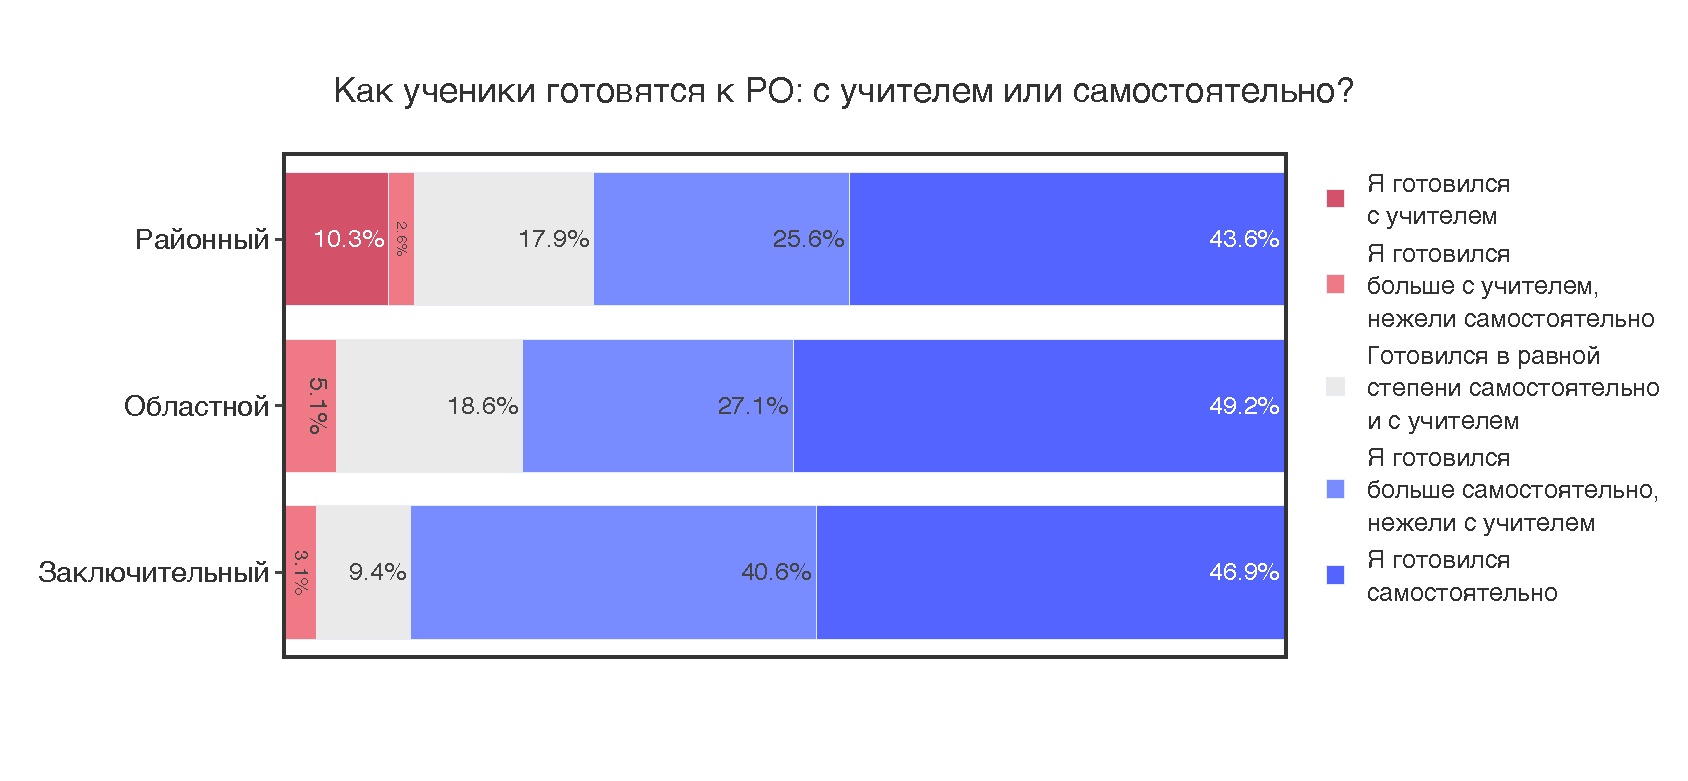
\includegraphics[width=\linewidth]{../export/pdf/demographics/prepstyle.pdf}


\section{Осведомленность о ресурсах}

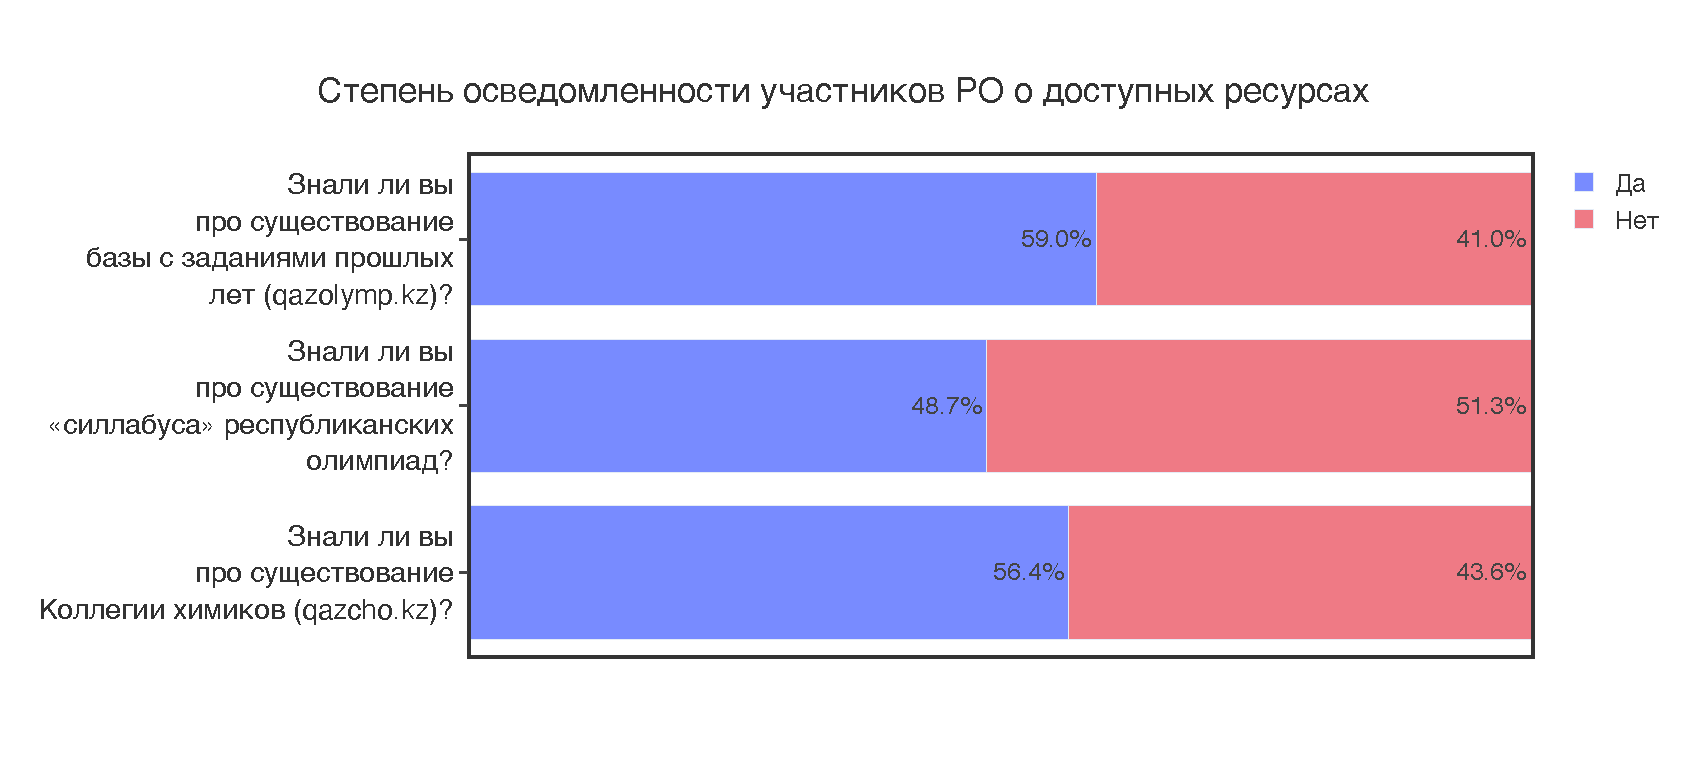
\includegraphics[width=\linewidth]{../export/pdf/demographics/shortquestions.pdf}

\textit{Примечание:} РНПЦ Дарын и Министерство Просвещения РК не предпринимали никаких попыток по распространению ресурсов, указанных ниже.

\section{Как готовились ученики}

Ученикам предлагалось ответить на следующий вопрос в открытой форме: \textit{Пожалуйста расскажите как вы готовились к республиканской олимпиаде. Какие интернет-ресурсы использовали? Какие учебники читали?}. Орфография и пунктуация авторов сохранены. Ответы собраны с 3 опросов (после каждого этапа РО). Представлена сводка наиболее репрезентативных ответов.

\begin{itemize}
    \itemsep-0.2em
    \item[--] Недавно начал использовать план подготовки от beyond по химии, а так решал задачи прошлых лет, по темам и тд.
    \item[--] Разные видео-уроки (youtube)
    \item[--] Изучаю механику органики по McMurry. Решал задания прошлых лет РО района и области, а также других олимпиад типа ОХО, на основании неизвестных заданий в этих олимпиадах искал материалы по ним в интернете
    \item[--] Мен тек ютубты қолдандым
    \item[--] Я Готовилась с учителем каждый день, готовилась со своего учебника, ходила на дополнительные, и решила задачи
    \item[--] beyond curriculum сайт. Книги: В. Ф. Травень ОРГАНИЧЕСКАЯ ХИМИЯ 1,2,3 том, и В. В. Еремин Теоретическая и математическая химия для школьников, В.В Ерёмин химия задачи 2400, макмюри(органика химия), Сорокин задачи.
    \item[--] Я использовал англоязычные книги, доступ к которым есть в интернете, я брал материалы именно с форума Спроси. Читал я "Органическую химию" Джона Макмюрри, и некоторые главы "Физической химии" Эткинса.
    \item[--] Смотрела онлайн уроки
    \item[--] По курсам по химии на https://www.lektorium.tv/, пробник ЕНТ по химии, задания Менделеевские, Всероссийские олимпиады прошлых лет.
    \item[--] Видео-ресурсы в YouTube, разные сайты, учебники
    \item[--] Решал респы/области прошлых лет, темы которые не знал читал в теормате и на Ютубе видео если в теормате не вникал, что происходит. Органику просто гуглил реакции и записывал механизмы в отдельную тетрадку, если реакция или похожая была в Клайдене, читал подглаву про реакцию.
\end{itemize}

Подавляющее большинство респондентов указывали набор наиболее широко известных книг и учебников, многие упоминали \href{https://olympiads.bc-pf.org}{план подготовки от Beyond Curriculum} и \href{https://ask.bc-pf.org/}{форум Спроси}. Коллегия была удивлена количеством учеников, которые ищут информацию на YouTube. Есть основания предполагать, что если поколение нынешних членов Коллегии искало неизвестную информацию в Google (например, "как подготовиться к республиканской олимпиаде" или "задания республиканской олимпиады по химии"), то нынешнее поколение делает этот запрос сразу в YouTube. Иными словами, ученики не находят существующие ресурсы, т.к. они не представлены в YouTube. Создание видеоматериалов, отвечающих на наиболее распространенные запросы пользователей, таким образом, может помочь с распространением информации о ресурсах, доступных для подготовки к республиканским олимпиадам.